\section{Internal Tests}

\subsection{GOAL Test Set}
First of all, let us see how many unsuccessful complementation tasks there were with the internal tests on the \goal{} test set. Table~\ref{i.g.out_table} shows the number of timeouts and memory excesses for each of the eight tested versions of the Fribourg construction.

\begin{table}[ht]
\centering
% latex table generated in R 3.1.2 by xtable 1.7-4 package
% Sat Jun  6 16:42:17 2015
\begin{tabular}{lrr}
  \hline
Construction & Timeouts & Memory excesses \\ 
  \hline
Fribourg & 48 & 0 \\ 
  Fribourg+R2C & 30 & 0 \\ 
  Fribourg+R2C+C & 54 & 0 \\ 
  Fribourg+M1 & 2 & 0 \\ 
  Fribourg+M1+M2 & 1 & 0 \\ 
  Fribourg+M1+R2C & 1 & 0 \\ 
  Fribourg+M1+R2C+C & 8 & 0 \\ 
  Fribourg+R & 48 & 0 \\ 
   \hline
\end{tabular}

\caption{Number of timeouts and memory excesses in the internal tests on the \goal{} test set.}
\label{i.g.out_table}
\end{table}

As we can see in the table, there were no memory excesses, that is, none of the 11,000 complementation tasks required more than 1 GB memory (actually, Java heap size). On the other hand, there is quite a number of timeouts. If we extract the effective samples from these result sets, we get a set of 10,939 automata. That means that these 10,939 automata have been successfully completed by all the versions of the Fribourg construction, whereas the remaining 61 automata (0.55\%) provoked a timeout in at least one of the versions.

Our main analysis is now about the sizes of the complements of these 10,939 automata. With size we mean the number of states of an automaton. A stripchart as the one in Figure~\ref{i.g.stripchart} is a good way to get a first glance of the complement sizes. Each horizontal strip contains 10,939 dots, each one corresponding to a produced complement automaton. The x-position of a dot indicates the size of the corresponding complement automaton.

\begin{figure}[ht]
\centering
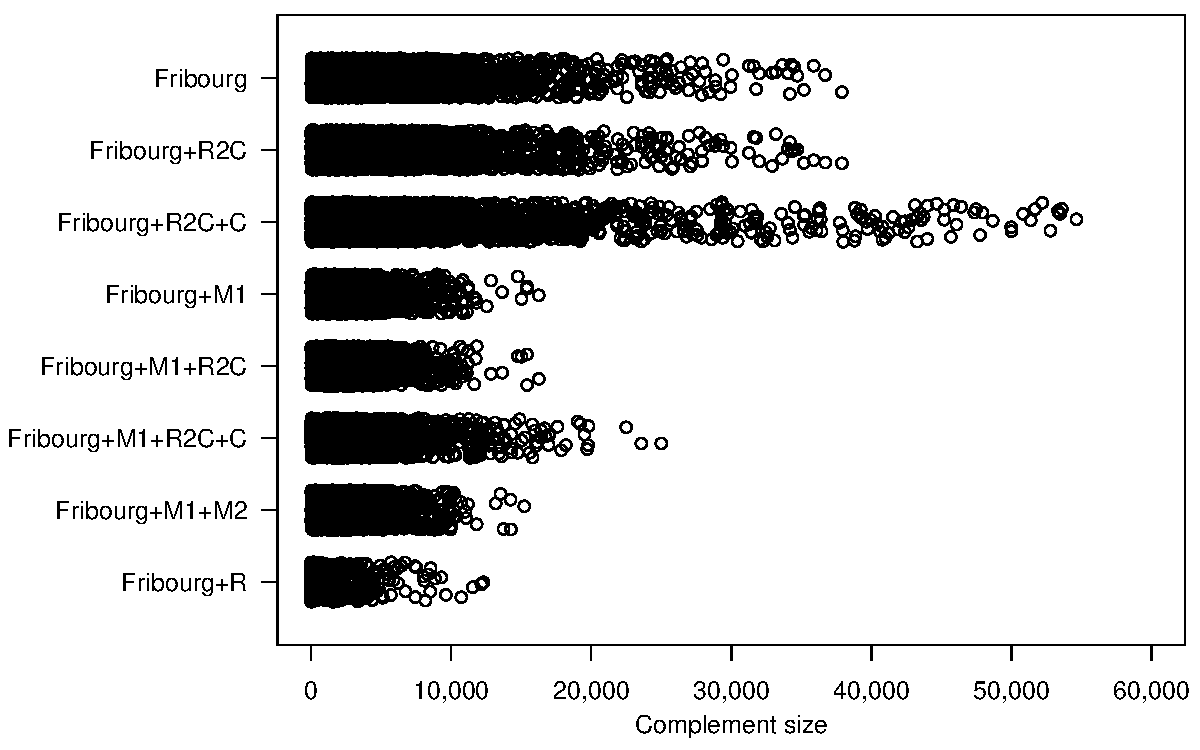
\includegraphics[width=0.7\textwidth]{figures/r/internal/goal/s.stripchart.pdf}
\caption{Stripchart with the complement sizes of the 10,939 effective samples of the \goal{} test set.}
\label{i.g.stripchart}
\end{figure}

The first thing to note is that the distribution of complement sizes is extremely right-skewed (also known as positive-skewed). The peak close to the left end of the x-axis and there is a long tail toward the right. This means that most of the complements are very small and the frequency decreases with increasing complement size. Finally, there are some few complements which are very large. This distribution implies that the mean is generally higher than the median, because the mean is ``dragged'' to the right by the few very large complements.

Next, we can compare the distributions of the individual version to each other. While Fribourg and Fribourg+R2C have a similarly long tail, Fribourg+R2C+C has a considerably longer one. This clearly is the effect of increasing the size of 91\% of the automata by adding a sink state in order to make them complete. Next, Fribourg+M1, Fribourg+M1+M2, and Fribourg+M1+R2C have similarly long tails that are significantly shorter than the ones of the previous versions. This indicates that the M1 optimisation is effective in reducing the size of otherwise large complements. Fribourg+M1+R2C+C, as expected, again increases the size of the tail due to the C option. Finally, Fribourg+R has a very short tail and an even higher concentration of very small complements. This is because the complements are pruned by removing their unreachable and dead states, and thus at least the complements of the 61.8\% universal input automata are reduced to empty automata of size 1.

Having a first impression of the distribution of complement sizes, we can look at some statistics characterising this distribution. Table~\ref{i.g.stats_table} shows the mean complement size along with the classic five-number summary consisting of minimum value, 25th percentile, median, 75th percentile and maximum value for each version of the Fribourg construction. As expected, the mean is always higher than the median. Generally, the median is a more robust metrics than the mean, because it is not affected by the value of outliers. This applies specifically to our distribution where some few very large complements might significantly increase the man whereas they leave the median unaffected. Therefore, the median will be our main metric, and the subsequent analyses will be based on the median.

\begin{table}[ht]
\centering
% latex table generated in R 3.1.2 by xtable 1.7-4 package
% Sat Jun  6 16:42:20 2015
\begin{tabular}{lrrrrrr}
  \hline
Construction & Mean & Min. & P25 & Median & P75 & Max. \\ 
  \hline
Piterman+EQ+RO & 209.6 & 1 & 38.0 & 80.0 & 183.0 & 20,349 \\ 
  Slice+P+RO+MADJ+EG & 949.4 & 2 & 120.0 & 396.0 & 1,003.0 & 41,081 \\ 
  Fribourg+M1+R2C & 1,017.3 & 2 & 153.0 & 452.0 & 1,134.0 & 37,068 \\ 
   \hline
\end{tabular}

\caption{Statistics of the complement sizes of the 10,939 effective samples of the \goal{} test set.}
\label{i.g.stats_table}
\end{table}

Going through the median values in Table~\ref{i.g.stats_table} we encounter some surprises. To begin with, as expected, there is a decrease from Fribourg (761) to Fribourg+R2C (689). Then, however, there is a significant drop to 451 with Fribourg+R2C+C. This is a surprise insofar as by looking at Figure~\ref{i.g.stripchart}, Fribourg+R2C+C seems to have the worst performance at a first glance. Indeed it also has the highest mean, which is due to the group of extremely large complements. The median, however, is very low, even lower than the one of Fribourg+M1 with its significantly shorter tail in Figure~\ref{i.g.stripchart}. Also the 25th percentile of Fribourg+R2C+C is with 85 one of the lowest. Going to the other side of the median, however, the 75th percentile (2,329) is the largest of all versions. A possible characterisation of this phenomenon is that the C option (together with R2C) makes small complements smaller, and large complements larger. The diminishment of small complements is far-reaching enough that the median is affected by it and decreased significantly.

The next thing we see in Table~\ref{i.g.stats_table} is that the median of Fribourg+M1 (482) is slightly lower than the median of Fribourg+M1+M2 (496). The same applies to the 25th and 75th percentile. This backs up our statement from Section~\ref{4_internal} that Fribourg+M1 performs better on the \goal{} teset set than Fribourg+M1+M2. The difference is rather small (the median increase is by 2.9\%), but it is enough to consider Fribourg+M1 as the better of the two versions, and to combine it therefore with R2C and R2C+C.

Fribourg+M1+R2C brings down the median from 482 to 447, with respect to Fribourg+M1. Also the 25th and 75th percentile are decreased. Adding the C option to Fribourg+M1+R2C, again causes the median to drop dramatically, from 447 to 331. The 25th percentile decreases from 152 to 83. The 75th percentile however increases from 1,118 to 1,208.5. Here we have again the same picture of the effecto of adding the C option that we had before. Namely that small complements are made smaller, and large complements are made larger.

Finally, the last row in Table~\ref{i.g.stats_table} with Fribourg+R shows the extent of unreachable and dead states that the Fribourg construction produces. The median is 1, and a further analysis reveals that the single-state complements go up to the 61st percentile. That is, 61\% of the complements have a size of 1. This is likely to correspond to the 61.8\% of universal automata in the GOAL test set whose complements can be reduced to empty automata with a single state.

% Time
% \begin{table}[ht]
% \centering
% % latex table generated in R 3.1.2 by xtable 1.7-4 package
% Wed Aug 19 09:24:28 2015
\begin{tabular}{LrrrrrrRr}
  \hline
Construction & Mean & Min. & P25 & Median & P75 & Max. & Total & $\approx$ hours \\ 
  \hline
Fribourg & 8.5 & 2.5 & 3.3 & 4.9 & 7.3 & 586.0 & 93,351.2 & 259 \\ 
  Fribourg+R2C & 6.6 & 2.2 & 2.9 & 4.2 & 6.4 & 219.7 & 72,545.7 & 202 \\ 
  Fribourg+R2C+C & 8.5 & 2.2 & 2.6 & 3.5 & 6.4 & 582.9 & 93,396.2 & 259 \\ 
  Fribourg+M1 & 4.9 & 2.5 & 3.2 & 4.1 & 5.9 & 55.1 & 54,061.3 & 150 \\ 
  Fribourg+M1+R2C & 4.4 & 2.2 & 2.8 & 3.6 & 5.3 & 42.5 & 48,572.0 & 135 \\ 
  Fribourg+M1+R2C+C & 5.6 & 2.5 & 3.2 & 4.0 & 6.5 & 147.4 & 60,918.9 & 169 \\ 
  Fribourg+M1+M2 & 4.6 & 2.2 & 2.9 & 3.8 & 5.1 & 38.4 & 49,848.0 & 138 \\ 
  Fribourg+R & 7.5 & 2.2 & 3.0 & 3.9 & 6.3 & 470.5 & 82,387.3 & 229 \\ 
   \hline
\end{tabular}

% \caption{Running times in seconds of the complementation tasks, measured as CPU time.}
% \end{table}
% \textcolor{red}{It is strange that Fribourg+R is so much faster than Fribourg}

Up to now, we only looked at statistics aggregated over the entire test set. But as we know from Section~\ref{4_goal_testset}, the 11,000 automata of the \goal{} test set are divided into 110 classes which consist of combinations of 11 transition densities and 10 acceptance densities. The transition densities range from 1 to 3 in steps of 0.2, and the acceptance densities range from 0.1 to 1 in steps of 0.1. In each class there are 100 automata. It is assumable that the median complement sizes are different for different classes. In the next step of the analysis, we want to analyse exactly this point. How do the median complement sizes of the different classes compare to each other, and can we identify a pattern of the classes that result in large and small complements?

This type of analysis naturally results in three-dimensional data. The classes themselves have two dimensions (the transition densities and the acceptance densities), and each of them has a third dimension consisting of the median complement size of this class. One way to present such data is by, for example, a 11x10 matrix with the rows being the transition densities, the columns the acceptance densities, and the cells the median values. Another way is by so called perspective plots. We used both of these ways in Section~\ref{4_goal_testset} when we analysed the number of complete and universal automata in each class of the \goal{} test set. In the present analysis, we will use perspective plots and omit the matrices for space reasons. However, we present the corresponding matrices in Appendix~\ref{app_matrices}. In this way, the interested reader may consult the exact values of the median complement sizes for each class. In the same way, we restrict ourselves to the median complement sizes as the third dimension. The same analysis could also be done, for example, for the mean, the 25th percentile, or the 75th percentile of complement sizes. However, as mentioned, we consider the median to be the most meaningful statistics, and thus exclusively focus on it for the matter of conciseness.

Figures~\ref{i.g.persp-1} and~\ref{i.g.persp_2} show the perspective plots of the median complement sizes for the 110 classes of the \goal{} test set. Each crossing of two lines on the xy-plane represents a class, and the z-value (height) of thie crossing indicates the median complement size of this class. As a help for the orientation, if one imagines the corresponding matrices, as they are presented in Appendix~\ref{app_matrices}, then in the perspective plots we are looking at these matrices from the bottom-right corner. That is, the class that is in the top-left corner of a matrix (transiton density 1.0 and acceptance density 0.1) is the one that is the farthest away from the viewer in the corresponding perspective plot. This orientation holds for all the remaining perspective plots in this thesis. The colours of the squares in the perspective plot (called facets) are a function of the z-values of their four corners and are selected to draw an analogy with topographical terrain maps.

\newcommand{\perspwidth}{0.475}

\begin{figure}[ht]
\centering
  \hfill
  \begin{subfigure}[t]{\perspwidth\textwidth}
  \centering
  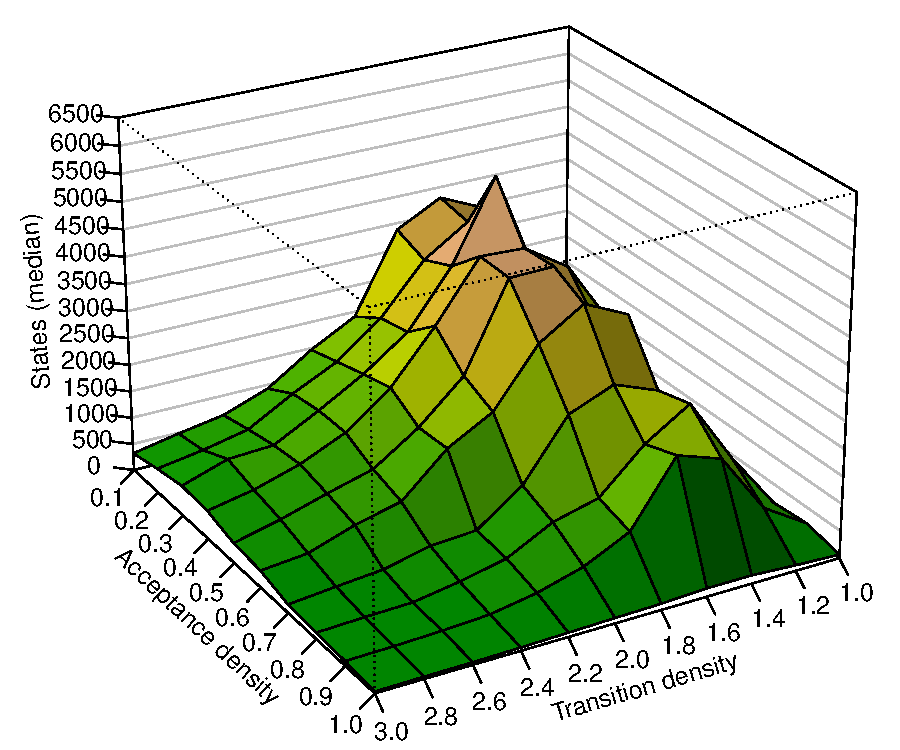
\includegraphics[width=\textwidth]{figures/r/internal/goal/s.median.Fribourg.pdf}
  \caption{Fribourg}
  \end{subfigure}
  \hfill
  \begin{subfigure}[t]{\perspwidth\textwidth}
  \centering
  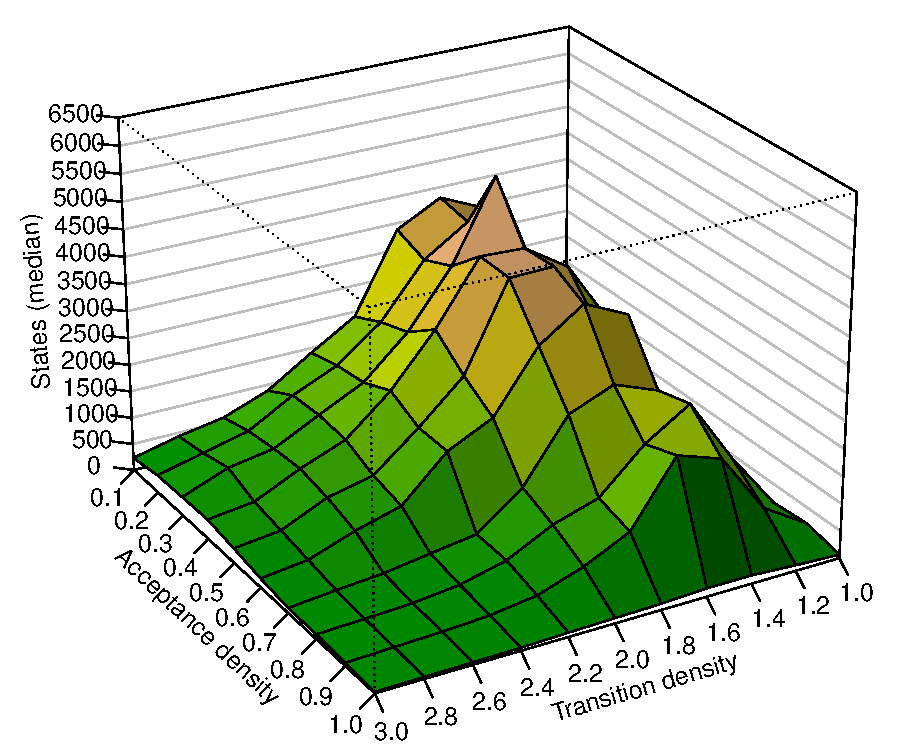
\includegraphics[width=\textwidth]{figures/r/internal/goal/s.median.Fribourg+R2C.pdf}
  \caption{Fribourg+R2C}
  \end{subfigure}
  \hfill

  \hfill
  \begin{subfigure}[t]{\perspwidth\textwidth}
  \centering
  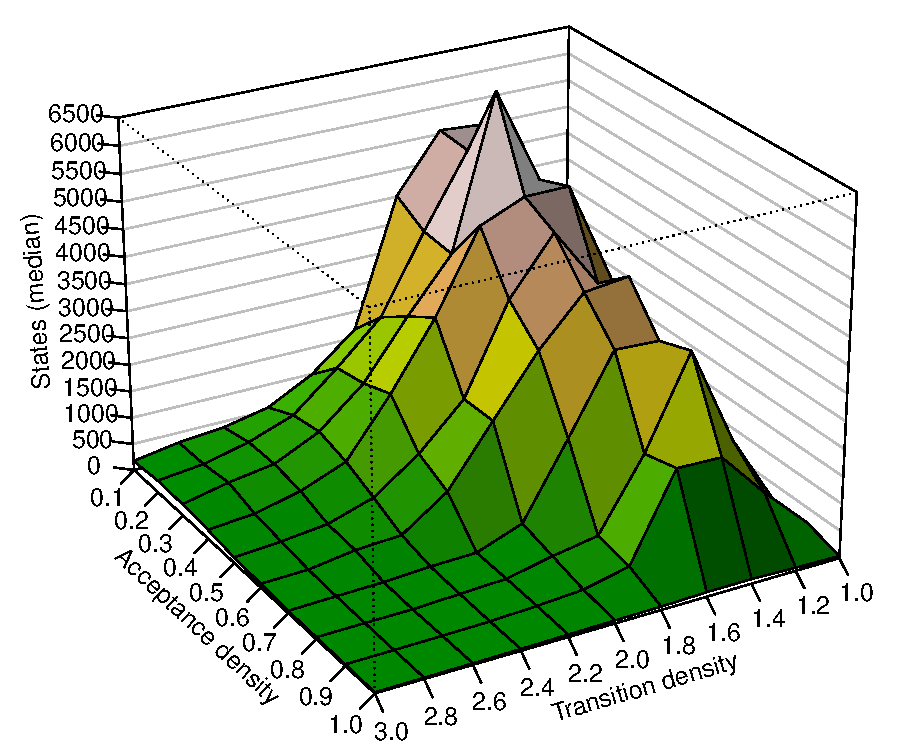
\includegraphics[width=\textwidth]{figures/r/internal/goal/s.median.Fribourg+R2C+C.pdf}
  \caption{Fribourg+R2C+C}
  \end{subfigure}
  \hfill
  \begin{subfigure}[t]{\perspwidth\textwidth}
  \centering
  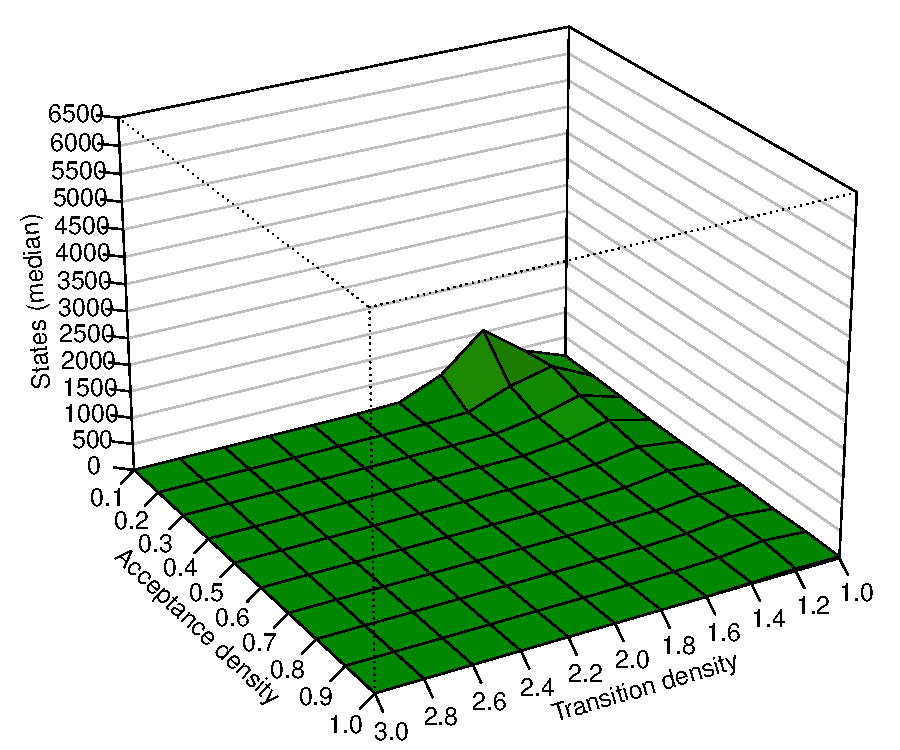
\includegraphics[width=\textwidth]{figures/r/internal/goal/s.median.Fribourg+R.pdf}
  \caption{Fribourg+R}
  \end{subfigure}
  \hfill  
\caption{Median complement sizes of the 110 transition density/acceptance density classes of the 10,939 effective samples of the \goal{} test set.}
\label{i.g.persp_1}
\end{figure}

The first thing we notice when looking at the plots in Figure~\ref{i.g.persp_1} and~\ref{i.g.persp_2} is that there are indeed large differences in the median complement sizes across the transition/acceptance density classes. Figuratively speaking, there is an oblong mountain (or hill) in the northern part of the area in east-west orientation, whose ridge increases in height from east to west and stays high until the western edge of the area. The mountain is located roughly in the area of transition densities between 1.2 and 2.2 and acceptance densities from 0.1 up to 0.9. This means that the automata of these classes are apparently harder to complement than the automata of other classes, as they result more frequently in larger complements.

We will further elaborate on the reasons of these different complement sizes across classes, and also try to characterise easy, medium, and hard automata for the Fribourg construction, at the end of this subsection. For now, we focus on the relative differences of median complement sizes between the different versions of the Fribourg construction.

Looking at Figure~\ref{i.g.persp_1}, the perspective plots for Fribourg and Fribourg+R2C are rather similar. The top of the mountain ridge is at between 3,500 and 4,000 states with a single peak of around 4900 states in the class with transition density 1.6 and acceptance density 0.3. From Table~\ref{i.g.stats_table} we can learn that the overall median complement size is 761 for Fribourg and 689 for Fribourg+R2C. These low values might surprise at first as the mountain, which is much higher, seems to dominate. However, by taking a closer look, it becomes apparent that around half of the classes are in rather low terrain (less than 1,000 states). Furthermore, the heights of the mountain peak do not allow to deduce anything about the overall median, because the median is not affected by the actual values of the data points which are greater than the median. This is the main characteristics of the median and applies to all the subsequent perspective plots in this chapter. The means in turn are 2,004.6 for Fribourg and 1955.9 for Fribourg+R2C.

Fribourg+R2C+C in Figure~\ref{i.g.persp_1} (c) has an even considerably higher mountain than the previous two versions. The top of the ridge is at around 5,000 states and the peak at the class with transition density 1.6 and acceptance density 0.3 has close to 6,500 states. This increase in height is however not reflected in the overall median of Fribourg+R2C+C relative to Fribourg+R2C. As we have seen in in Table~\ref{i.g.stats_table}, the median of Fribourg+R2C+C is 451, and thus 34.5\% lower than the median of Fribourg+R2C. By taking a closer look at the perspective plots, the reason for this can be seen, as the low areas of Fribourg+R2C+C are indeed slightly lower than the low areas of Fribourg+R2C. The significantly higher high areas of Fribourg+R2C+C do not have an effect on the overall median. However, they do have an effect on the overall mean which with 2,424.6 is indeed 24\% higher than the one of Fribourg+R2C (1,955.9).

Going from the first three perspective plot in Figure~\ref{i.g.persp_1} to the perspective plot of Fribourg+R is like going from the Swiss Alps to a Dutch polder. The mountain shrinks to a small hillock and the rest of the terrain is low and flat. This is because so many complements of the Fribourg construction can be reduced to very small sizes by removing their unreachable and dead states. A look at the corresponding matrix in Appendix~\ref{app_matrices} reveals that 68 of the 110 classes have a median complement size of 1. If we further compare this matrix to the matrix with the number of universal automata in Figure~\ref{4_compl_univ} (b), we see that all the classes with a median of 1 contain more than 50 universal automata, and the classes with a median greater than 1 contain less than 50 universal automata. There is a total of 100 automata per class. This makes sense as the complements of universal automata are empty automata, and every empty automaton can be reduced to an automaton with a single non-accepting state. Looking at the classes with a median greater than 1, we see that their values are still considerably lower than the ones of the plain Fribourg construction, which indicates that the Fribourg construction generates a large number of unreachable and dead states. However, as already mentioned, this thread of analysis is not the focus of the present thesis, and we leave it for future work.

\begin{figure}[ht]
\centering
  \hfill
  \begin{subfigure}[t]{\perspwidth\textwidth}
  \centering
  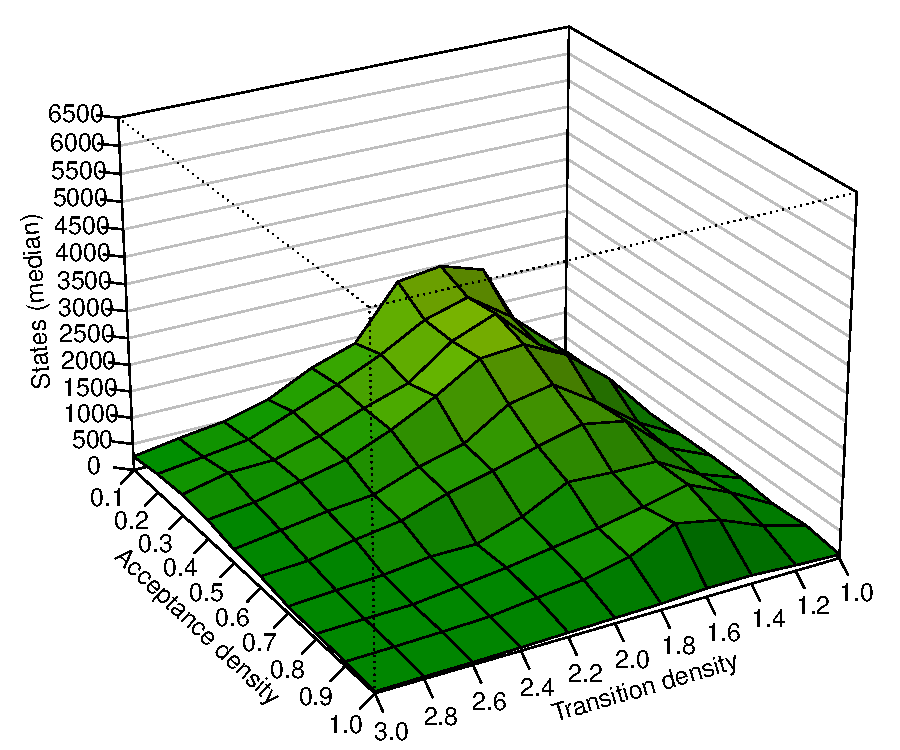
\includegraphics[width=\textwidth]{figures/r/internal/goal/s.median.Fribourg+M1.pdf}
  \caption{Fribourg+M1}
  \end{subfigure}
  \hfill
  \begin{subfigure}[t]{\perspwidth\textwidth}
  \centering
  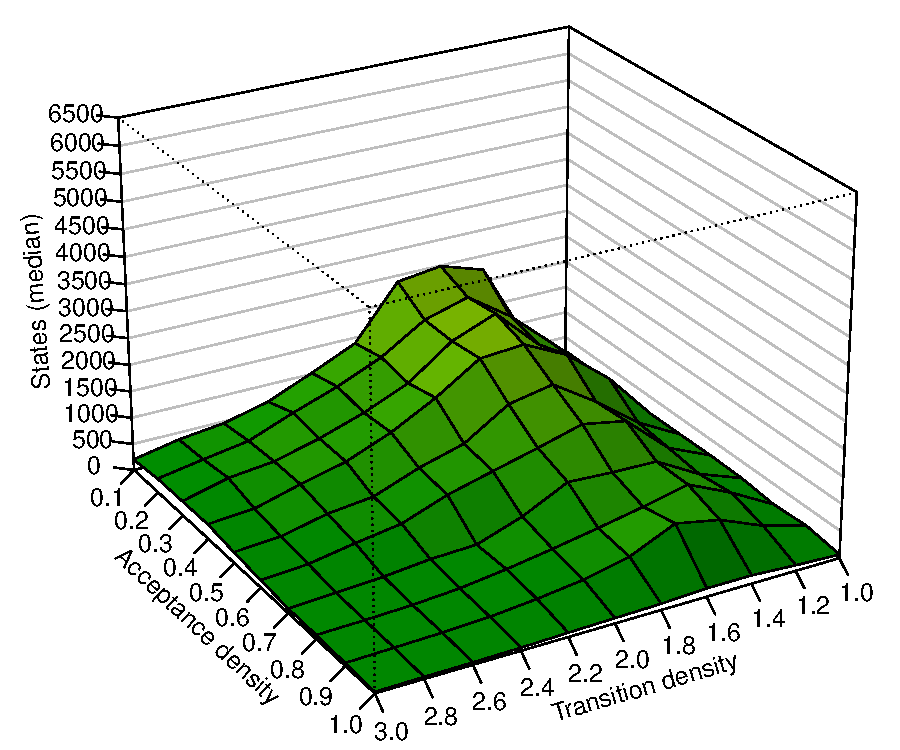
\includegraphics[width=\textwidth]{figures/r/internal/goal/s.median.Fribourg+M1+R2C.pdf}
  \caption{Fribourg+M1+R2C}
  \end{subfigure}
  \hfill

  \hfill
  \begin{subfigure}[t]{\perspwidth\textwidth}
  \centering
  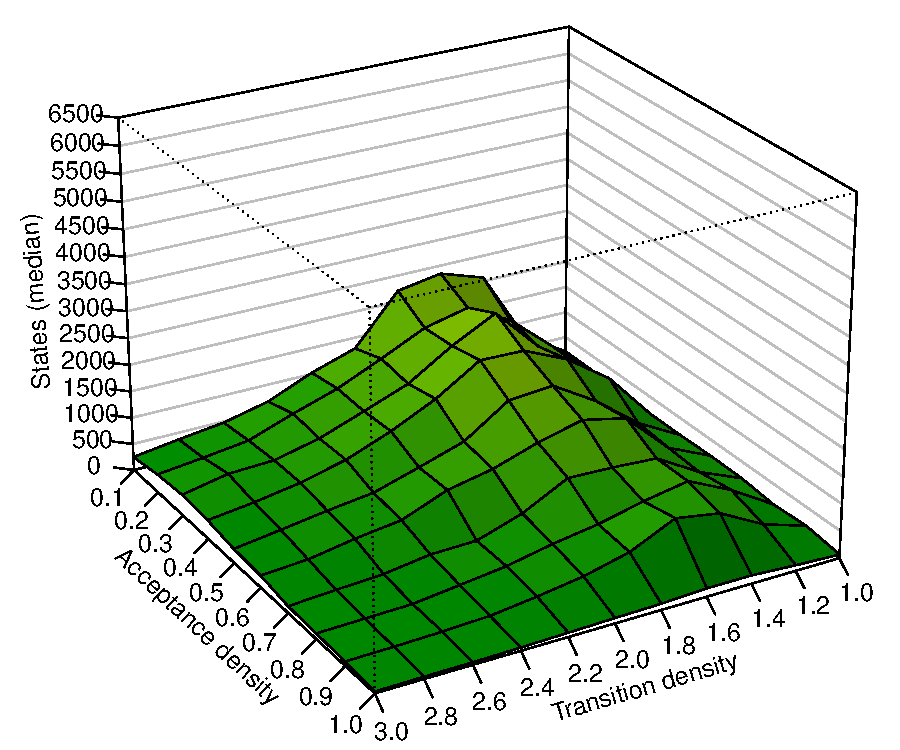
\includegraphics[width=\textwidth]{figures/r/internal/goal/s.median.Fribourg+M1+M2.pdf}
  \caption{Fribourg+M1+M2}
  \end{subfigure}
  \hfill
  \begin{subfigure}[t]{\perspwidth\textwidth}
  \centering
  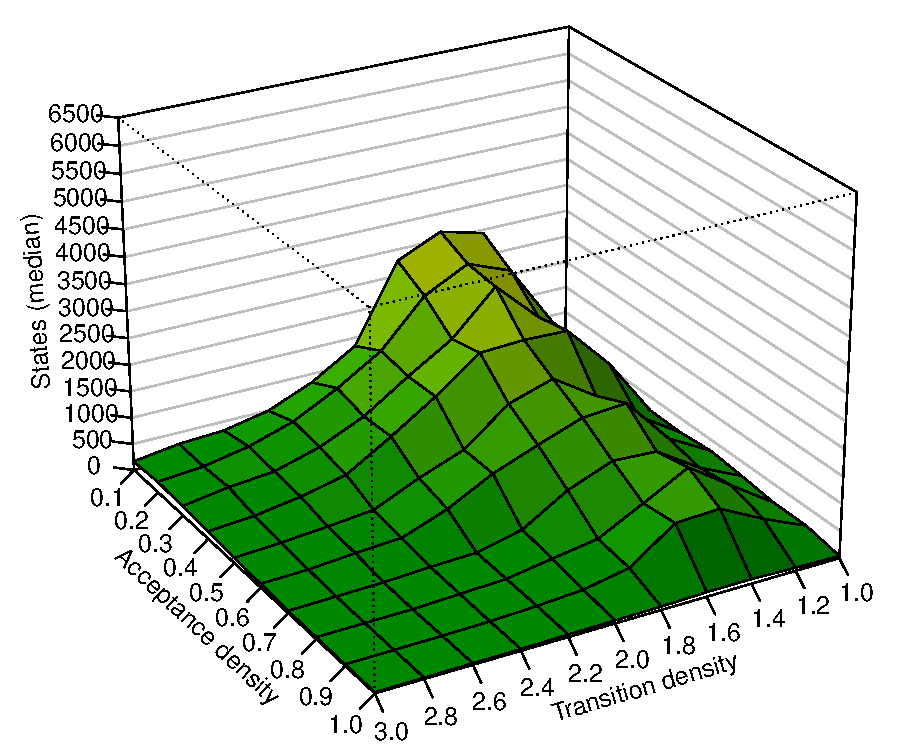
\includegraphics[width=\textwidth]{figures/r/internal/goal/s.median.Fribourg+M1+R2C+C.pdf}
  \caption{Fribourg+M1+R2C+C}
  \end{subfigure}
  \hfill
\label{i.g.persp_2}
\end{figure}

Figure~\ref{i.g.persp_2} shows the perspective plots of the remaining four versions of the Fribourg construction, all of which include the M1 optimisation. The first thing we note is that, while the mountain is still there, its height shrinks significantly. For Fribourg+M1, and Fribourg+M1+R2C, the top of the ridge is between is around 2,500 states. This is reflected by the overall means of these two versions compared to their counterparts without the M1 optimisation, Fribourg, and Fribourg+R2C. The decrease of the overall mean from Fribourg to Fribourg+M1 is by 52\% (from 2004.6 to 963.2) and from Fribourg+R2C to Fribourg+M1+R2C by 52.1\% (from 1955.9 to 937.7). The decreases of the overall medians are by 36.6\% (from 761 to 482), and 35.1\% (from 689 to 447) for the same two pairs of versions. With this we can confirm that the M1 optimisation brings a significant performance gain. 

Regarding the M2 optimisation, we can see that the mountain ridge in the Fribourg+M1+M2 perspective plot is slightly lower than the one in the Fribourg+M1 perspective plot. The flatland regions, however, seem to not change much. This is reflected by the overall mean of Fribourg+M1+M2 which is slightly lower than in Fribourg+M1 (958.9 opposed to 963.2). The overall median, on the other hand, is higher for Fribourg+M1+M2 than for Fribourg+M1 (496 opposed to 482). An interpretation of this behaviour is that the application of the M2 optimisation results in smaller complements for \textit{some} input automata. These automata are especially the ``hard'' ones that produce large complements. This positive effect of M2 does however not affect enough input automata, especially not the ``easy'' automata, as to improve the overall performance of the construction in terms of median complement size. As already stated previously, we consider therefore Fribourg+M1 as the better construction on the \goal{} test set than Fribourg+M1+M2.

Finally,Fribourg+M1+R2C+C differs from Fribourg+M1+R2C in a similar way Fribourg+R2C+C differs from Fribourg+R2C. The higher regions get higher and the lower regions get lower, that is, a performance decline on ``hard'' automata, but a performance gain on easy automata. The performance gain on the easy automata is however effective enough to decrease the overall median from 447 to 331, which is minus 26\%.

With 331 states, Fribourg+M1+R2C+C has the lowest median of all the versions (except Fribourg+R which is a special case because it modifies the output of the construction). However, we still declare Fribourg+M1+R2C as the winner on the \goal{} test set, mainly for two reasons. First, while Fribourg+M1+R2C+C has a lower median, the mean is still higher (1062.6 to 937.7 which is a plus of 13.3\%). This results from the complements of the hard automata, which are larger than with Fribourg+M1+R2C. From a practical point of view, the mean might be relevant, because it relates more directly to the required computing resources than the median. For example the execution CPU time per complementation task, that we also measured along with our experiments, is 25.4\% higher for Fribourg+M1+R2C+C than for Fribourg+M1+R2C. The increase in the average execution time per automaton is from 4.44 to 5.57 seconds and in the total execution time from 48,572 seconds ($\approx$ 135 hours) to 60,919 seconds ($\approx$ 169 hours). Fribourg+M1+R2C, on the other hand, has the lowest mean of all versions. The second reason that we choose Fribourg+M1+R2C as the winner and not Fribourg+M1+R2C+C is that the C option is not a real part of the construction. It actually modifies the input automata before the construction starts in order to make them better suited for the construction. Fribourg+M1+R2C, on the other hand, includes only native options, and input and output of the construction are not modified. This should also make it fairer to compare the Fribourg construction to other constructions in the external tests (Section~\ref{ext}).

As we have seen, there are big difference in the complement sizes across the different classes of the \goal{} test set. Furthermore, there is a certain pattern, namely the mountain in the north-western region of the class matrix. Automata of classes that are in the mountain region seem to be harder to complement than automata from the classes in the flatland region. We attempted to categorise the classes of the \goal{} test set into the three groups ``easy'', ``medium'', and ``hard''. To do so, we first averaged the matrices with the median complement sizes of all the eight versions of the Fribourg construction. In this way, we have a mean median complement size for each class. Then we defined two breakpoints that divide the classes into easy, medium, and hard groups. The breakpoints 500 and 1,600 result in an appropriate groups that seem to capture the reality well. The result with these breakpoints can be seen in Figure~\ref{i.g.difficulty}.

\begin{figure}[ht]
\centering
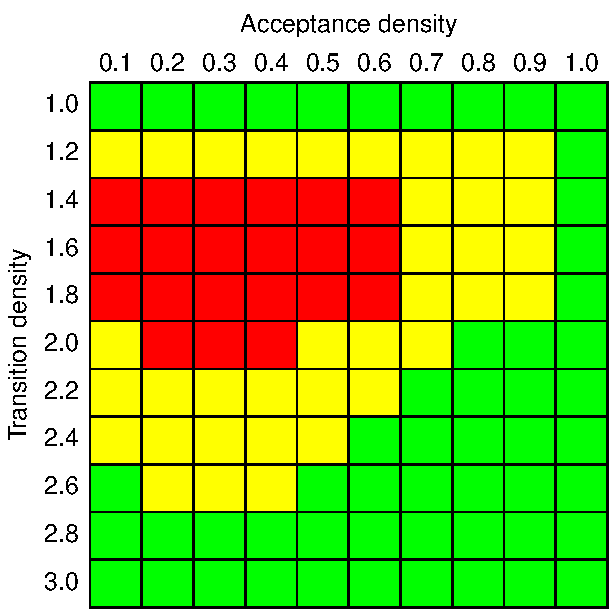
\includegraphics[width=0.35\textwidth]{figures/r/internal/goal/difficulty.pdf}
\caption{Difficulty categories of the transition/acceptance density classes of the \goal{} test set. Green: easy; yellow: medium; red: hard.}
\end{figure}

As can be seen in Figure~\ref{i.g.difficulty}, there are 53 easy, 36 medium, and 21 hard classes. The easy classes are mainly those with extreme values. In particular, all the classes with a low or high transition density of 0.1, or 2.8 and 3.0, and a high acceptance density of 1.0 are easy. Furthermore, there is a ``triangle'' of easy classes between transition densities 2.0 and 2.6. and acceptance densities 0.5 and 0.9. The higher the transition density, the lower the acceptance density may be so that the corresponding class is still easy. The hard classes are roughly those with a transition density between 1.4 and 1.8 and an acceptance density between 0.1 and 0.6. The medium classes finally are situated as a ``belt'' around the hard classes.

It is interesting that the extreme values of transition density and acceptance density result in easy automata. With a transition density of 1.0 and an alphabet size of 2, each of the 15 states has on average two outgoing and two incoming transitions\footnote{The transition density multiplied with the number of states defines the number of transition for each symbol of the alphabet in the automaton, see Section~\ref{4_goal_testset}.}. With a transition density of 3.0, each state has on average 6 outgoing and 6 incoming transitions. These low or high connectivity seems to considerably simplify the complementation task. The same applies to a high acceptance density of 1.0, which means that every state is an accepting state\footnote{The acceptance density defines the percentage of states that are accepting, see Section~\ref{4_goal_testset} as well.}. Generally, we can say that automata with high acceptance densities are easier to complement than automata with lower acceptance densities. This also means that the pattern of easy automata at the extreme values of transition and accceptance density, does not apply to to the lower extreme of the acceptance density. Automata with a very low acceptance density of 0.1 are hard to complement---unless they are made easy by a low or high transition density.

Another interesting point is that the hard automata have transition densities between 1.4 and 1.8. It seems that this range of transition densities is the crucial factor in the hardness of a complementation task, and that it is only alleviated by a growing acceptance density. This explains the decline of the mountain ridge from west to east.

Summarising we can say that transition densities between 1.4 and 1.8 produce the hardest complementation tasks, and that to the both sides the difficulty steadily decreases with declining or growing transition density. Furthermore, a growing acceptance density generally implies easier complementation tasks.


\subsection{Michel Test Set}
We complemented the first four Michel automata with the six versions of the Fribourg constructions that are listed in Section~\ref{4_internal}. All complementation tasks were successful, as we did not set a timeout or memory limit. Remember that the first four Michel automata have 3, 4, 5, and 6 states, respectively. The sizes of the resulting complements are presented in Figure~\ref{i.m.states} in table form and visualised as a grouped barplot.

\begin{figure}[ht]
  \centering
  \begin{subtable}{0.75\textwidth}
    \centering
    % latex table generated in R 3.1.2 by xtable 1.7-4 package
% Sun Aug 16 00:19:45 2015
\begin{tabular}{lrrrrrr}
  \hline
Construction & Michel 1 & Michel 2 & Michel 3 & Michel 4 & Fitted curve & Std. error \\ 
  \hline
Fribourg & 57 & 843 & 14,535 & 287,907 & $(1.35n)^n$ & 0.01\% \\ 
  Fribourg+R2C & 33 & 467 & 8,271 & 168,291 & $(1.24n)^n$ & 0.06\% \\ 
  Fribourg+M1 & 44 & 448 & 5,506 & 81,765 & $(1.10n)^n$ & 0.07\% \\ 
  Fribourg+M1+M2 & 42 & 402 & 4,404 & 57,116 & $(1.03n)^n$ & 0.12\% \\ 
  Fribourg+M1+M2+R2C & 28 & 269 & 3,168 & 43,957 & $(0.99n)^n$ & 0.04\% \\ 
  Fribourg+R & 18 & 95 & 528 & 3,315 & $(0.64n)^n$ & 0.35\% \\ 
   \hline
\end{tabular}

  \end{subtable}

  \begin{subfigure}{0.7\textwidth}
    \centering
    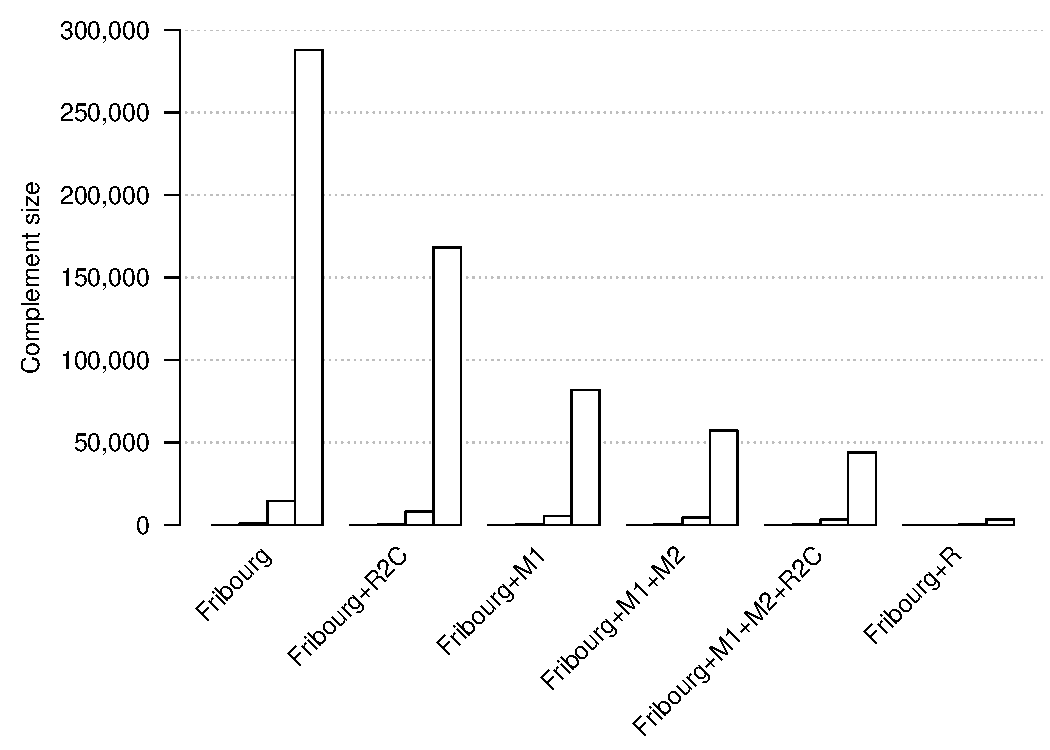
\includegraphics[width=\textwidth]{figures/r/internal/michel/s.barplot.pdf}
    \caption{Complement sizes of the first four Michel visualised as a barplot. The bars 1 to 4 of each group correspond to Michel automata 1 to 4.}
  \end{subfigure}
\caption{Complement sizes of the Michel automata in table form and visualised as a barplot. Each version of the Fribourg construction is represented by four bars, which stand for Michel automata 1 to 4, respectively.}
\label{i.m.states}
\end{figure}

Looking at the results reveals two things. First, Michel automata result in very large complements. For example, Michel 4, which has six states, results in a complement with 287,907 states with the plain Fribourg construction. This is a state growth of $(1.354n)^n$. Exactly this state explosion is the aim of Michel automata, which have been developed with the goal to crate a set of automata that is extremely hard to complement.

This also shows why we were only able to complement the first four Michel automata. If we assume the same state growth of $(1.354n)^n$ for the fifth Michel automaton, Michel 5, with seven states, then the complement would have around 6.9 million states. The execution time for Michel 4 with the plain Friboug construction was 100,976 CPU time seconds ($\approx$ 180 hours). If we assume a linear relation between the number of generated states and the execution time, then Michel 5 would have an execution time of more than 2.4 million seconds, which is around 279 days. This estimation is still a very conservative, as the relation between complement size and execution time is not linear but seems to be exponential as well (see table with exeuction times in appendix). 




\section{External Tests}
\label{ext}

\subsection{GOAL Test Set}

\begin{table}[ht]
\centering
% latex table generated in R 3.1.2 by xtable 1.7-4 package
% Sat Jun  6 16:42:17 2015
\begin{tabular}{lrr}
  \hline
Construction & Timeouts & Memory excesses \\ 
  \hline
Fribourg & 48 & 0 \\ 
  Fribourg+R2C & 30 & 0 \\ 
  Fribourg+R2C+C & 54 & 0 \\ 
  Fribourg+M1 & 2 & 0 \\ 
  Fribourg+M1+M2 & 1 & 0 \\ 
  Fribourg+M1+R2C & 1 & 0 \\ 
  Fribourg+M1+R2C+C & 8 & 0 \\ 
  Fribourg+R & 48 & 0 \\ 
   \hline
\end{tabular}

\caption{Number of timeouts and memory excesses.}
\end{table}

\begin{itemize}
\item With Rank
  \begin{itemize}
  \item 7,204 effective samples (3,796 uncompleted tasks, 34.51\%)
  \end{itemize}
\item Without Rank
  \begin{itemize}
  \item 10,998 effective samples (2 uncompleted tasks, 0.02\%)
  \end{itemize}
\end{itemize}


\subsubsection{With Rank}

\begin{figure}[ht]
\centering
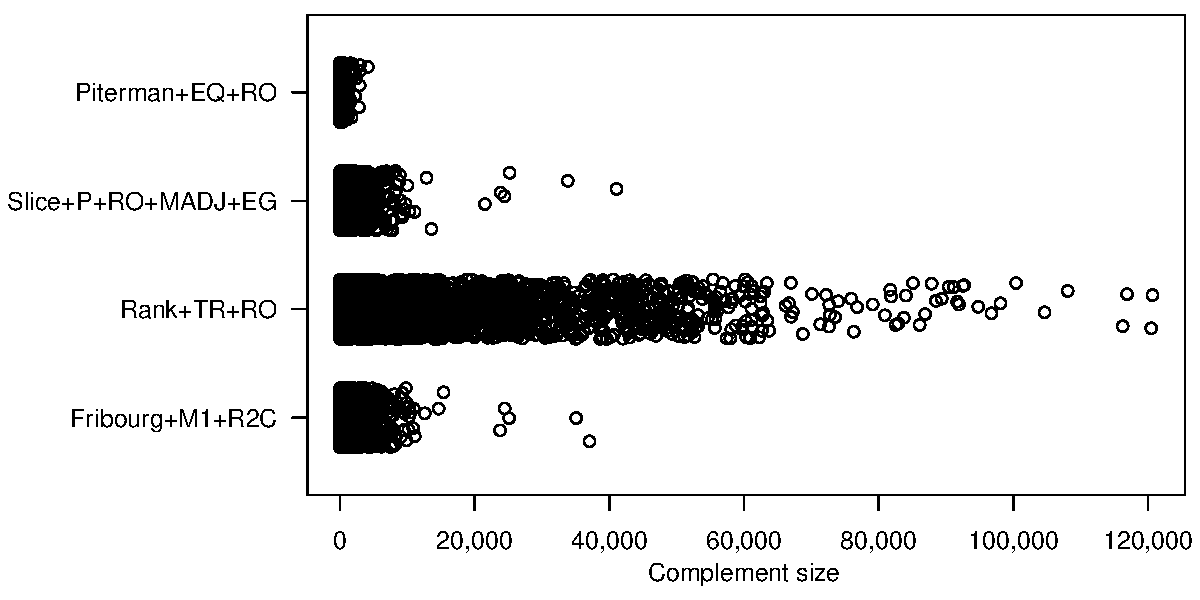
\includegraphics[width=0.75\textwidth]{figures/r/external/goal/s.stripchart.with_rank.pdf}
\caption{Complement sizes of the 7,204 effective samples.}
\end{figure}

\begin{table}[ht]
\centering
% latex table generated in R 3.1.2 by xtable 1.7-4 package
% Sun Aug 16 15:57:19 2015
\begin{tabular}{lrrrrrr}
  \hline
Construction & Mean & Min. & P25 & Median & P75 & Max. \\ 
  \hline
Piterman+EQ+RO & 106.0 & 1 & 29.0 & 58.0 & 121.0 & 4,126 \\ 
  Slice+P+RO+MADJ+EG & 555.4 & 2 & 70.0 & 202.0 & 596.0 & 41,081 \\ 
  Rank+TR+RO & 5,255.6 & 2 & 81.0 & 254.5 & 3,178.2 & 120,674 \\ 
  Fribourg+M1+R2C & 662.9 & 2 & 101.0 & 269.0 & 754.5 & 37,068 \\ 
   \hline
\end{tabular}

\caption{Aggregated statistics of complement sizes of the 7,204 effective samples.}
\end{table}

\begin{table}[ht]
\centering
% latex table generated in R 3.1.2 by xtable 1.7-4 package
% Thu Jun 11 15:11:29 2015
\begin{tabular}{lrrrrrr}
  \hline
Construction & Mean & Min. & P25 & Median & P75 & Max. \\ 
  \hline
Piterman+EQ+RO & 2.97 & 2.22 & 2.58 & 2.78 & 3.03 & 42.93 \\ 
  Slice+P+RO+MADJ+EG & 3.66 & 2.21 & 2.69 & 3.22 & 4.07 & 36.67 \\ 
  Rank+TR+RO & 16.04 & 2.28 & 2.76 & 3.71 & 9.31 & 443.33 \\ 
  Fribourg+M1+R2C & 4.02 & 2.22 & 2.69 & 3.10 & 4.37 & 410.37 \\ 
   \hline
\end{tabular}

\caption{Aggregated statistics of the running times of the 7,204 effective samples.}
\end{table}


\subsubsection{Without Rank}


\begin{figure}[ht]
\centering
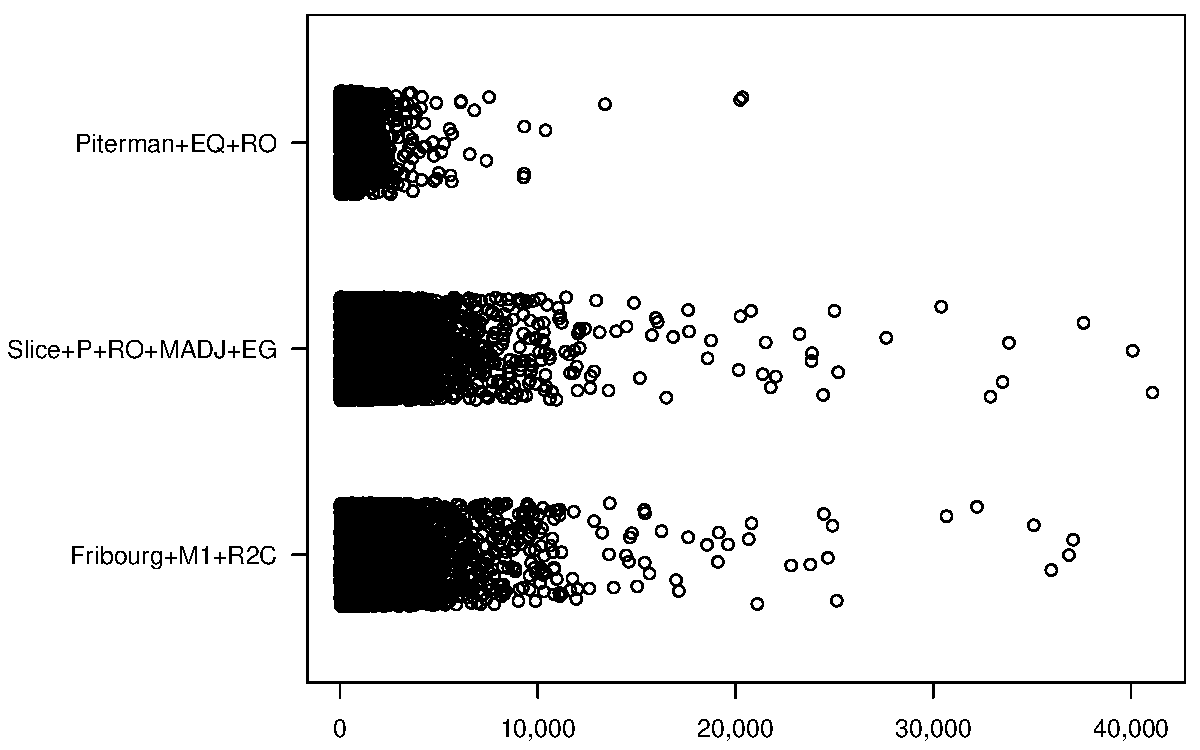
\includegraphics[width=0.75\textwidth]{figures/r/external/goal/s.stripchart.pdf}
\caption{Complement sizes of the 10,998  effective samples.}
\end{figure}


\begin{table}[ht]
\centering
% latex table generated in R 3.1.2 by xtable 1.7-4 package
% Sat Jun  6 16:42:20 2015
\begin{tabular}{lrrrrrr}
  \hline
Construction & Mean & Min. & P25 & Median & P75 & Max. \\ 
  \hline
Piterman+EQ+RO & 209.6 & 1 & 38.0 & 80.0 & 183.0 & 20,349 \\ 
  Slice+P+RO+MADJ+EG & 949.4 & 2 & 120.0 & 396.0 & 1,003.0 & 41,081 \\ 
  Fribourg+M1+R2C & 1,017.3 & 2 & 153.0 & 452.0 & 1,134.0 & 37,068 \\ 
   \hline
\end{tabular}

\caption{Aggregated statistics of complement sizes of the 10,998 effective samples without Rank.}
\end{table}

\begin{table}[ht]
\centering
% latex table generated in R 3.1.2 by xtable 1.7-4 package
% Wed Aug 19 09:24:28 2015
\begin{tabular}{LrrrrrrRr}
  \hline
Construction & Mean & Min. & P25 & Median & P75 & Max. & Total & $\approx$ hours \\ 
  \hline
Fribourg & 8.5 & 2.5 & 3.3 & 4.9 & 7.3 & 586.0 & 93,351.2 & 259 \\ 
  Fribourg+R2C & 6.6 & 2.2 & 2.9 & 4.2 & 6.4 & 219.7 & 72,545.7 & 202 \\ 
  Fribourg+R2C+C & 8.5 & 2.2 & 2.6 & 3.5 & 6.4 & 582.9 & 93,396.2 & 259 \\ 
  Fribourg+M1 & 4.9 & 2.5 & 3.2 & 4.1 & 5.9 & 55.1 & 54,061.3 & 150 \\ 
  Fribourg+M1+R2C & 4.4 & 2.2 & 2.8 & 3.6 & 5.3 & 42.5 & 48,572.0 & 135 \\ 
  Fribourg+M1+R2C+C & 5.6 & 2.5 & 3.2 & 4.0 & 6.5 & 147.4 & 60,918.9 & 169 \\ 
  Fribourg+M1+M2 & 4.6 & 2.2 & 2.9 & 3.8 & 5.1 & 38.4 & 49,848.0 & 138 \\ 
  Fribourg+R & 7.5 & 2.2 & 3.0 & 3.9 & 6.3 & 470.5 & 82,387.3 & 229 \\ 
   \hline
\end{tabular}

\caption{Aggregated statistics of the running times of the 10,998 effective samples without Rank.}
\end{table}

% Persp plots
\renewcommand{\perspwidth}{0.3}

\begin{figure}[ht]
\centering
  \hfill
  \begin{subfigure}[t]{\perspwidth\textwidth}
  \centering
  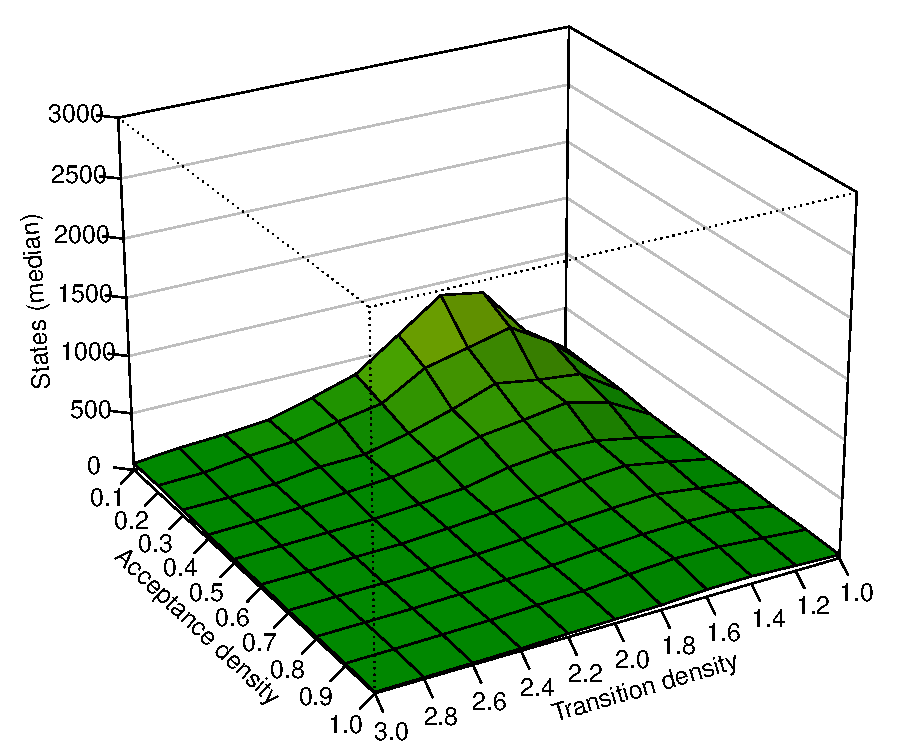
\includegraphics[width=\textwidth]{figures/r/external/goal/s.median.Piterman+EQ+RO.pdf}
  \caption{Piterman+EQ+RO}
  \end{subfigure}
  \hfill
  \begin{subfigure}[t]{\perspwidth\textwidth}
  \centering
  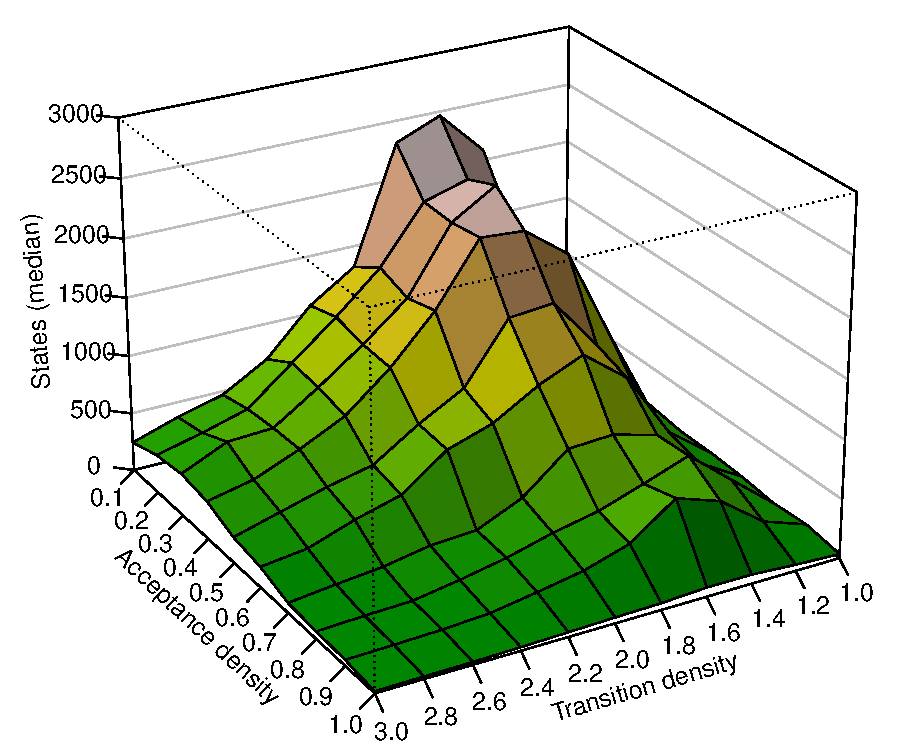
\includegraphics[width=\textwidth]{figures/r/external/goal/s.median.Slice+P+RO+MADJ+EG.pdf}
  \caption{Slice+P+RO+MADJ+EG}
  \end{subfigure}
  \hfill
  \begin{subfigure}[t]{\perspwidth\textwidth}
  \centering
  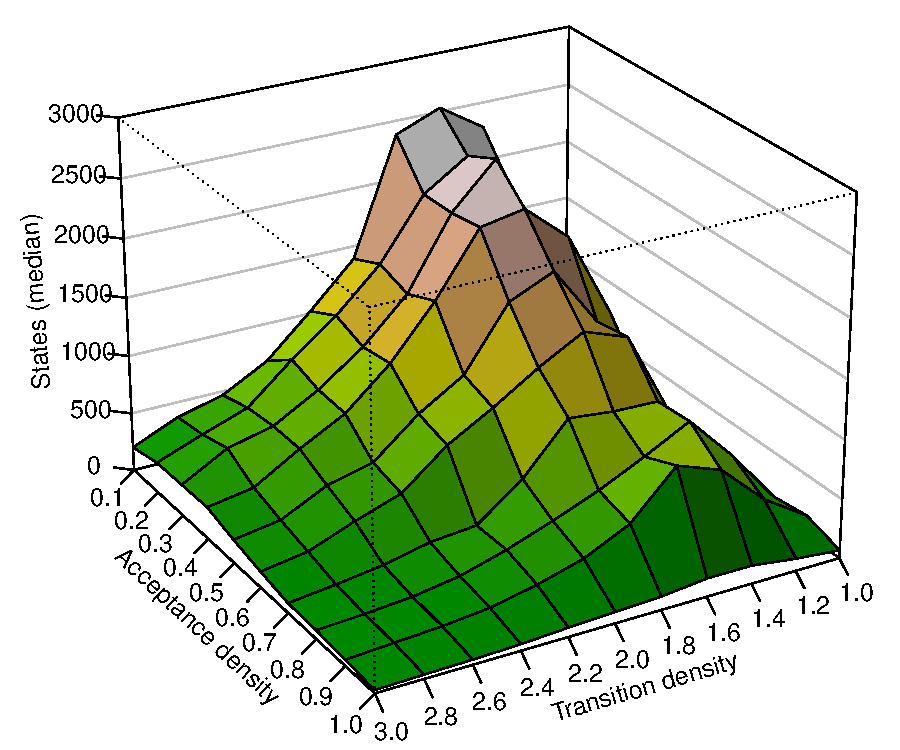
\includegraphics[width=\textwidth]{figures/r/external/goal/s.median.Fribourg+M1+R2C.pdf}
  \caption{Fribourg+M1+R2C}
  \end{subfigure}
  \hfill
\caption{Median complement sizes.}
\end{figure}



\subsection{Michel Automata}




\begin{figure}[ht]
  \centering
  \begin{subtable}{0.75\textwidth}
    \centering
    % latex table generated in R 3.1.2 by xtable 1.7-4 package
% Sun Aug 16 00:19:45 2015
\begin{tabular}{lrrrrrr}
  \hline
Construction & Michel 1 & Michel 2 & Michel 3 & Michel 4 & Fitted curve & Std. error \\ 
  \hline
Fribourg & 57 & 843 & 14,535 & 287,907 & $(1.35n)^n$ & 0.01\% \\ 
  Fribourg+R2C & 33 & 467 & 8,271 & 168,291 & $(1.24n)^n$ & 0.06\% \\ 
  Fribourg+M1 & 44 & 448 & 5,506 & 81,765 & $(1.10n)^n$ & 0.07\% \\ 
  Fribourg+M1+M2 & 42 & 402 & 4,404 & 57,116 & $(1.03n)^n$ & 0.12\% \\ 
  Fribourg+M1+M2+R2C & 28 & 269 & 3,168 & 43,957 & $(0.99n)^n$ & 0.04\% \\ 
  Fribourg+R & 18 & 95 & 528 & 3,315 & $(0.64n)^n$ & 0.35\% \\ 
   \hline
\end{tabular}

    \caption{Complement sizes of the first four Michel automata.}
  \end{subtable}

  \begin{subfigure}{0.75\textwidth}
    \centering
    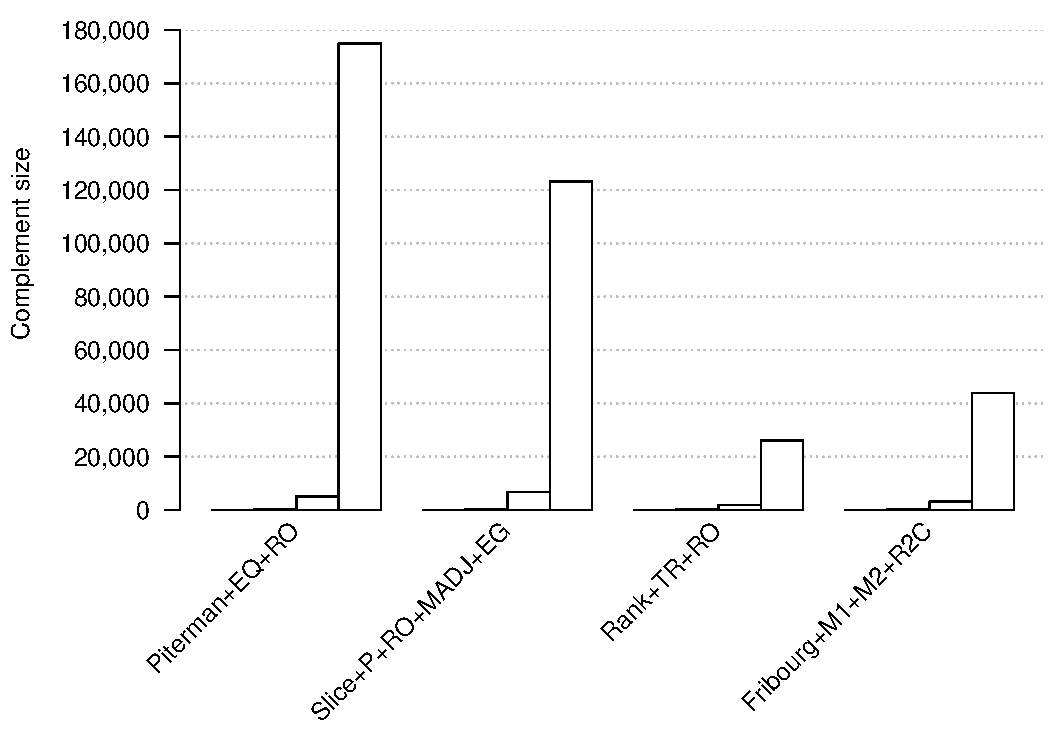
\includegraphics[width=\textwidth]{figures/r/external/michel/s.barplot.pdf}
    \caption{Complement sizes of the first four Michel visualised as a barplot. The bars 1 to 4 of each group correspond to Michel automata 1 to 4.}
  \end{subfigure}
  \caption{Complement sizes of Michel automata.}
\end{figure}


\begin{table}[ht]
\centering
% latex table generated in R 3.1.2 by xtable 1.7-4 package
% Sun Aug 16 00:19:45 2015
\begin{tabular}{lrrrrrr}
  \hline
Construction & Michel 1 & Michel 2 & Michel 3 & Michel 4 & Fitted curve & Std. error \\ 
  \hline
Fribourg & 57 & 843 & 14,535 & 287,907 & $(1.35n)^n$ & 0.01\% \\ 
  Fribourg+R2C & 33 & 467 & 8,271 & 168,291 & $(1.24n)^n$ & 0.06\% \\ 
  Fribourg+M1 & 44 & 448 & 5,506 & 81,765 & $(1.10n)^n$ & 0.07\% \\ 
  Fribourg+M1+M2 & 42 & 402 & 4,404 & 57,116 & $(1.03n)^n$ & 0.12\% \\ 
  Fribourg+M1+M2+R2C & 28 & 269 & 3,168 & 43,957 & $(0.99n)^n$ & 0.04\% \\ 
  Fribourg+R & 18 & 95 & 528 & 3,315 & $(0.64n)^n$ & 0.35\% \\ 
   \hline
\end{tabular}

\caption{Execution times for the first four Michel automata.}
\end{table}
